\section{Lab 1: Configurazione di una rete su Linux}
\subsection{Introduzione}
Supponiamo di avere il seguente scenario:
\begin{figure}[H]
    \centering
    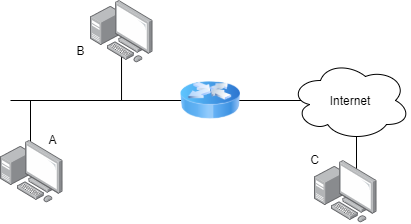
\includegraphics[width=300px]{images/1.1_Configurazione_di_una_rete_Linux/simple_network.png}
\end{figure}
se volessimo configurare uno qualsiasi degli host dovremmo conoscere queste 4 informazioni:
\begin{itemize}
    \item Indirizzo IP
    \item Subnet Mask
    \item Gateway address
    \item DNS address
\end{itemize}

\subsubsection{Indirizzo IP}
E' un numero a 32 bit che individua una scheda di rete all' interno di una sottorete.
Per comodità anziché ricordare i 32 bit singolarmente si usa la notazione puntata, si prendono i 4 ottetti singolarmente e li si scrivono in decimale separati da un punto.

\begin{verbatim}
    11000000101010000000000101000110
        192 .  168  .   1    .   70
\end{verbatim}
Un indirizzo IP è diviso in due porzioni:
\begin{figure}[H]
    \centering
    
\includegraphics[width=200px]{images/1.1_Configurazione_di_una_rete_Linux/ip_parts.png}
\end{figure}
In base a dove decidiamo di inserire il limite tra le due porzioni possiamo avere reti più o meno grandi, questo è utile per poter segmentare l' intero range di indirizzi IP.
Se ho più bit per la rete posso creare più reti diverse, se ho più bit per gli host posso inserire più host diversi nella stessa sottorete.

\subsubsection{Subnetmask}
E' un insieme di 32 bit in cui i primi $x$, usati per indicare i bit della rete, sono tutti a 1 ed i rimanenti tutti a 0.
Come dice il nome è una maschera che si può usare assieme all' indirizzo IP per trovare:
\begin{itemize}
    \item indirizzo della rete: AND logico tra IP e netmask
    \item indirizzo di broadcast: OR logico tra IP e netmask \emph{negata}
\end{itemize}

\subsection{Comando ip}
Per avere a che fare con le configurazioni di rete su Linux si usa il tool \emph{ip}, questo tool è omnicomprensivo a differenza della suite che si usava fino a pochi anni fa che metteva a disposizione vari tool per fare configurazioni diverse che però avevano sempre a che fare con la rete.

\subsubsection{Ottenere informazioni sulle interfacce}
\begin{verbatim}
    $ ip addr show
    $ ip a show
    $ ip a
\end{verbatim}
si usano per ottenere le configurazioni correntemente in funzione.
Vediamo di cosa si compone un esempio di output:
\begin{verbatim}
    2: eth0: <BROADCAST,MULTICAST,UP,LOWER_UP> mtu 1500 qdisc
    pfifo_fast state UP group default qlen 1000
        link/ether 08:00:27:9b:5c:4d brd ff:ff:ff:ff:ff:ff
        inet 192.168.1.52/24 brd 192.168.1.255 scope global
    dynamic noprefixroute eth0
           valid_lft 21596sec preferred_lft 21596sec
        inet6 fe80::ccbe:5117:5e99:2b07/64 scope link
    noprefixroute 
           valid_lft forever preferred_lft forever
\end{verbatim}

\begin{itemize}
    \item 2: numero dell' interfaccia nell' elenco
    \item eth0: nome dell' interfaccia
    \item $<$BROADCAST,MULTICAST,UP,LOWER\_UP$>$: ci dice che questa connessione permette la comunicazione in broadcast, multicast e che l' interfaccia è accesa ed anche il cavo è connesso
    \item mtu 1500: Maximum Transmission Unit, massima grandezza in byte dei frame che possono essere inviati attraverso questa interfaccia
    \item qdisc fq\_codel: queueing discipline, politica di invio dei pacchetti in coda, in questo caso pfifo\_fast cioè una normale coda FIFO
    \item state UP: stato dell' interfaccia
    \item qlen 1000: lunghezza massima della coda
    \item link/ether 08:00:27:9b:5c:4d : è l' indirizzo MAC (fisico) della periferica
    \item brd ff:ff:ff:ff:ff:ff : è l' indirizzo MAC del broadcast
    \item inet 192.168.1.52/24: indirizzo IP e subnet mask configurata sulla interfaccia 
    \item brd 192.168.1.255: indirizzo di broadcast della rete
    \item scope global: la visibilità di questa interfaccia è globale nella rete locale, quindi tutti gli altri host possono contattarla
\end{itemize}

\subsubsection{Abilitare e disabilitare le interfacce}
\begin{verbatim}
    # ip link set <interface> up
    # ip link set <interface> down
\end{verbatim}

\subsubsection{Impostare un IP ad una interfaccia}
\begin{verbatim}
    # ip a add <IP>/<CIDR> broadcast <broadcast IP> dev <interface>
\end{verbatim}

\subsubsection{Rimuovere un IP da una interfaccia}
\begin{verbatim}
    # ip a del <IP>/<CIDR> dev <interface>
    # ip a flush dev <interface>
\end{verbatim}
NB: questa configurazione si perde al riavvio!

\subsubsection{Configurazione permanente}
Per ottenere una configurazione permanente la si deve inserire nel file \emph{/etc/network/interfaces} usando i comandi \emph{ifup} e \emph{ifdown} appartenenti alla suite \emph{ifupdown}:
\begin{verbatim}
    auto lo
        # elenco delle interfacce da abilitare
        # e configurare all'avvio
        
    iface lo inet loopback
        # configura l'interfaccia lo come interfaccia di loopback
    
    iface eth0 inet static
        # configura l'interfaccia eth0 con
        # una configurazione statica
        address 192.168.1.2
            # specifica l'indirizzo IP
        netmask 255.255.255.0
            # specifica la netmask
        broadcast 192.168.1.255
            # specifica l'indirizzo di broadcast
\end{verbatim}
Per attivare la configurazione si usa:
\begin{verbatim}
    ifup eth0
\end{verbatim}
Prenderà la configurazione inserita nel file e la applicherà.
Per attivare tutte le interfacce elencate nel campo "auto" del file e nello stesso ordine:
\begin{verbatim}
    ifup -a
\end{verbatim}
Per disattivarla usiamo:
\begin{verbatim}
    ifdown eth0
\end{verbatim}

\subsection{Default gateway}
Quando un host deve inviare un pacchetto esegue il seguente algoritmo per capire come farlo:
\begin{itemize}
    \item calcolo la subnet del destinatario
    \item se è uguale alla subnet in cui è una delle interfacce del calcolatore
    \begin{itemize}
        \item invio direttamente il pacchetto
    \end{itemize}
    \item altrimenti
    \begin{itemize}
        \item invio il pacchetto verso il default gateway, cioè il router della nostra rete
    \end{itemize}
\end{itemize}
Per configurare il default gateway all'interno del file di configurazione si usa la linea:
\begin{verbatim}
    gateway <default gateway IP>
\end{verbatim}

\subsection{Tabelle di routing}
Le tabelle di routing sono delle tabelle che contengono i percorsi che faranno i pacchetti se devono andare verso un host conosciuto, una sottorete conosciuta ma anche verso host e reti sconosciute, attravero le route di default.

\subsubsection{Vedere le route}
Per visualizzare le tabelle di routing si usa il comando:
\begin{verbatim}
    $ ip route show
\end{verbatim}
e l'output è del tipo:
\begin{verbatim}
    default via 192.168.1.1 dev eth0
    192.168.1.0/24 dev eth0 ... src 192.168.1.2
\end{verbatim}
la prima in particolare ci dice che se l'host destinatario non è nella nostra sottorete i paccheti verrano inviati verso quell'IP usando quella interfaccia.

\subsubsection{Aggiungere una route}
\begin{verbatim}
    # ip route add 192.168.1.0/24 dev eth0
\end{verbatim}
Es: se devi mandare pacchetti nella rete 192.168.1.0 inviali sulla interfaccia eth0.

\subsubsection{Aggiungere una route default}
\begin{verbatim}
    # ip route add default via 192.168.1.1
\end{verbatim}
Es: se non sai dove inviare i pacchetti inviali a 192.168.1.1.

\subsubsection{Ottenere la route verso un indirizzo}
\begin{verbatim}
    $ ip route get 70.143.3.67
\end{verbatim}

\subsection{Traduzione di hostname e DNS}
Le traduzioni manuali possono essere aggiunte al sistema all'interno del file \emph{/etc/hosts}:
\begin{verbatim}
    127.0.0.1       localhost
    127.0.1.1       studenti
    151.101.241.140 www.reddit.com
\end{verbatim}

Le traduzioni dinamiche invece si eseguono tramite richieste a qualche Local DNS, per istruire il sistema operativo su quali server usare si compila il file \emph{/etc/resolv.conf}:
\begin{verbatim}
    nameserver 8.8.8.8
    nameserver 8.8.4.4
\end{verbatim}

Per ottenere una risoluzione in maniera manuale si usa il tool \emph{nslookup}:
\begin{verbatim}
    $ nslookup nome_dominio
\end{verbatim}
I sistemi UNIX per ottenere delle traduzioni usano NSS (Name Server Switch), per configurare l' ordine si deve modificare il file \emph{/etc/nsswitch.conf}:
\begin{verbatim}
    ...
    hosts: files dns
        # cerca prima nel file hosts e poi nel DNS
    ...
\end{verbatim}

\subsection{DHCP}
Se non voglio o non posso configurare i singoli host nella rete attraverso dei file statici posso fare ricorso al protocollo DHCP - \emph{Dynamic Host Configuration Protocol}.
Questo protocollo prevede l' inserimento di un server all' interno della rete opportunamente configurato per negoziare gli IP agli host che dovessero richiederli tramite il protocollo stesso.
Oltre a fornire l'indirizzo IP permette di configurare subnet mask, DNS e default gateway, in questo modo l' host è pronto per navigare nella rete senza necessità di configurazioni manuali. 

\subsubsection{Protocollo}
Appena connetto un cavo ethernet ad un host o lo connetto alla rete tramite il wifi:
\begin{itemize}
    \item il client invia una richiesta DHCPDISCOVER usando come indirizzo sorgente 0.0.0.0:68 e come indirizzo destinatario 255.255.255.255:67, in pratica il broadcast della rete in cui pensa di essere
    
    \item il server risponde con una DHCPOFFER con sorgente il suo vero indirizzo IP e come destinazione 255.255.255.255:68. All' interno della proposta abbiamo almeno:
    \begin{itemize}
        \item YADDR: indirizzo IP proposto
        \item lease time: tempo di scadenda dell'IP proposto
    \end{itemize}
    
    \item il client risponde con una DHCPREQUEST accettando la proposta
    
    \item il server risponde con un DHCPACK in modo da confermare la ricezione dell' accettazione
\end{itemize}
In una rete possono esserci anche più server DHCP in tal caso il client che riceve le offerte ne accetta una e declina tutte le altre.

\subsubsection{Installazione del server}
Sulla macchina debian per installare il server occorrono:
\begin{verbatim}
    # apt update
        ; aggiornare l'elenco dei repository
    # apt-get install isc-dhcp-server
        ; installazione del server
\end{verbatim}

\subsubsection{Configurazione del server}
Per configurare il server occorre modificare il file \emph{/etc/default/isc-dhcp-server} inserendo l' interfaccia del server sulla quale ascoltare per eventuali richieste.
\begin{verbatim}
    INTERFACES="eth0"
\end{verbatim}

All' interno del file \emph{/etc/dhcp/dhcpd.conf} invece si trova la configurazione della pool di IP che il server può allocare, assieme al DNS, al default gateway ed al lease time da propagare.
\begin{verbatim}
    option domain-name-servers 1.1.1.1, 1.0.0.1;
    option routers 10.0.2.2;
    
    default-lease-time 3600;
    
    subnet 10.0.2.0 netmask 255.255.255.0 {
        range 10.0.2.101 10.0.2.150;
    }
\end{verbatim}

Una volta configurato il server per rendere effettiva la configurazione occorre riavviare il servizio:
\begin{verbatim}
    # systemctl restart isc-dhcp-server.service
\end{verbatim}

\subsubsection{Configurazione del client}
Per permettere al client di configurarsi in automatico, occorre specificarlo nel file di configurazione \emph{/etc/network/interfaces}:
\begin{verbatim}
    iface eth0 inet dhcp
\end{verbatim}

\subsection{ICMP}
ICMP - \emph{Internet Control Message Protocol} è un protocollo di servizio al livello di rete usato per fini di diagnostica e statistica.

\subsubsection{Ping}
Usando una ICMP ECHO REQUEST un host chiede ad un altro host di rispondergli tramite una ICMP ECHO REPLY.
Possiamo eseguire queste richieste usando il tool \emph{ping}:
\begin{verbatim}
    $ ping www.apple.com
    $ ping 192.168.2.34
\end{verbatim}
Se l' host è presente, è attivo ed ha le richieste abilitate ci risponderà.
Il comando ping invia una serie di richieste, misura il tempo necessario a ricevere una risposta e ce lo stampa a schermo, inoltre ci conta il numero di pacchetti persi, cioè i pacchetti che hanno impiegato tempo maggiore del timeout per arrivare o che non sono arrivati proprio.
\begin{verbatim}
    PING apPlE.it (17.253.144.10) 56(84) bytes of data.
    64 bytes from seminars.apple.com (17.253.144.10): 
        icmp_seq=1 ttl=50 time=29.1 ms
    64 bytes from apple.com.do (17.253.144.10): icmp_seq=2
        ttl=50 time=30.1 ms
    64 bytes from apple.com.do (17.253.144.10): icmp_seq=3
        ttl=50 time=30.6 ms
    64 bytes from apple.de (17.253.144.10): icmp_seq=4
        ttl=50 time=32.3 ms
    64 bytes from podcast.apple.com (17.253.144.10):
        icmp_seq=5 ttl=50 time=30.4 ms
    64 bytes from icloud.com (17.253.144.10): icmp_seq=6
        ttl=50 time=29.7 ms
    64 bytes from apple.com.tt (17.253.144.10): icmp_seq=7
        ttl=50 time=34.5 ms
    64 bytes from apple.com.pa (17.253.144.10): icmp_seq=8
        ttl=50 time=30.0 ms
\end{verbatim}
Per stoppare il programma si può usare la shortcut: CTRL+C.

NB: se si vuole specificare il numero di richieste da eseguire:
\begin{verbatim}
    $ ping www.apple.com -c 10
\end{verbatim}

\subsubsection{Traceroute}
E' un comando che fornisce l' elenco degli host incontrati nel percorso da sorgente a destinazione.
In una rete di router esiste un algoritmo distribuito che calcola lo shortest path quando si chiede una destinazione.
Il concetto di percorso più breve è legato a qualche metrica, nelle reti se ne usano varie:
\begin{itemize}
    \item numero di hop: si contano il numero di router da attraversare prima di arrivare a destinazione, il percorso più breve è quello che passa per meno hop.
    In questo modo ogni arco ha peso unitario.
    
    \item distanza geografica: il percorso più breve può essere quello che è anche geograficamente più corto.
    In questo modo ogni arco ha un peso proporzionale alla lunghezza del media che connette i due router.
    
    \item percorso meno congestionato: se in una rete tutti i pacchetti prendono lo stesso percorso la rete potrebbe saturarsi, una ulteriore metrica prevede quindi di contemplare lo sfruttamento dei singoli link di connessione e dare un costo minore a quelli più liberi.
    In questo caso i pesi sugli archi sono dinamici e cambiano in base allo stato della rete, questa metrica è utile per distribuire il carico sulla rete.
\end{itemize}
Spesso anziché usare una singola metrica si cerca una ottimizzazione su più fattori: \emph{multi-objective optimization}.

Il comando traceroute funziona attraverso il campo TTL (time-to-live) dei pacchetti IP: un campo che contiene il numero di hop che il pacchetto può ancora fare prima di essere droppato. 
Ogni host che riceve il pacchetto prima di re-inviarlo, se non è lui il destinatario, deve diminuire il valore di questo campo e successivamente può inviare il pacchetto.
Se nel decrementare il valore scende a 0 l' host deve droppare il pacchetto e notificare la sorgente del mancato recapito, questa notifica è eseguita tramite un pacchetto \emph{time-exceeded} con all' interno anche l' IP di chi lo sta mandando.

Per funzionare quindi traceroute invia 3 pacchetti con TTL a 1, aspetta le risposte, successivamente invia 3 pacchetti con TTL a 2 e così via finché non si vede rispondere con un pacchetto \emph{ICMP destination unreachable}, questo è il destinatario che si accorge che la porta richiesta dal pacchetto non è connessa ad alcun processo.

Può ovviamente accadere che i 3 pacchetti inviati prendano percorsi diversi e quindi portino a risposte da IP differenti, per limitare il danno il software invia i 3 pacchetti quasi simultaneamente.

Analiziamo un output di esempio del programma:
\begin{verbatim}
    $ traceroute www.google.com
    traceroute to www.google.com (216.58.205.196), 30 hops max,
        60 byte packets
    1 131.114.175.73 (131.114.175.73) 0.348 ms 0.351 ms 0.378 ms
    2 jser-jing.unipi.it (131.114.191.129) 0.363 ms 0.371 ms
        0.398 ms
    3 ru-unipi-rx1-pi1.pi1.garr.net (193.206.136.13) 1.302 ms
        1.312 ms 1.321 ms
    4 rx1-pi1-rx2-mi2.mi2.garr.net (90.147.80.210) 6.881 ms
        6.899 ms 6.898 ms
    5 72.14.214.105 (72.14.214.105) 7.023 ms 6.974 ms 6.986 ms
    6 * * *
    7 216.239.42.27 (216.239.42.27) 7.020 ms 6.931 ms 6.997 ms
    8 mil04s29-in-f4.1e100.net (216.58.205.196) 6.949 ms 7.090
        ms 7.087 ms
\end{verbatim}
Per quasi ogni hop abbiamo:
\begin{itemize}
    \item hop count: numero di hop
    \item hostname della macchina che ha risposto
    \item IP dell' hop
    \item 3 valori di round-trip-time
\end{itemize}
Per alcuni hop possiamo avere il valore "*" per uno o più dei valori della terna, questo può succedere perchè:
\begin{itemize}
    \item il pacchetto si è perso all' andata
    \item il pacchetto si è perso al ritorno
    \item scadenza del timeout di 5s
    \item l'host ha le risposte ICMP disabilitate
    \item presenza di un firewall che limita il traffico
\end{itemize}



